\section{Rozwój postaci gracza w grach (Bartosz Strzelecki)}\label{s:wpr_progres}
Rozwój postaci gracza ma ogromne znaczenie w wielu wymiarach. Jest podstawowym elementem, dzięki któremu gracz może odczuwać postęp podczas rozwoju linii fabularnych. 
Stanowi to też nagrodę dla gracza, za poniesioną głęboką osobistą inwestycję wczuwając się w rolę postaci. Przez to ta mechanika pozytywnie
wpływa na motywację użytkownika do dalszych zmagań i pozwala na ponowne rozegranie gry, dzięki temu, że gracz może chcieć przejść
ponownie przez linię fabularną, podejmując inne decyzje podczas rozwijania postaci.

Jednym z wyróżniających aspektów serii gier The Elder Scrolls jest zaimplementowany system rozwoju postaci, który pozwala na różnorodne
przebiegi rozgrywki dynamicznie dostosowujące się do stylu preferowanego przez gracza. W skrócie, jeśli gracz preferuje strzelanie z łuku,
w trakcie rozgrywki będzie mógł rozwijać tę umiejętność, aby czerpać z niej jak najwięcej korzyści. Głęboka złożoność tego systemu sprzyja długoterminowemu zaangażowaniu,
dzięki czemu gracze poświęcają dużo więcej czasu na doskonalenie swoich postaci, odkrywanie nowych kombinacji umiejętności i eksperymentowaniem z różnymi
stylami rozgrywki.

\begin{figure}[h]
\centering
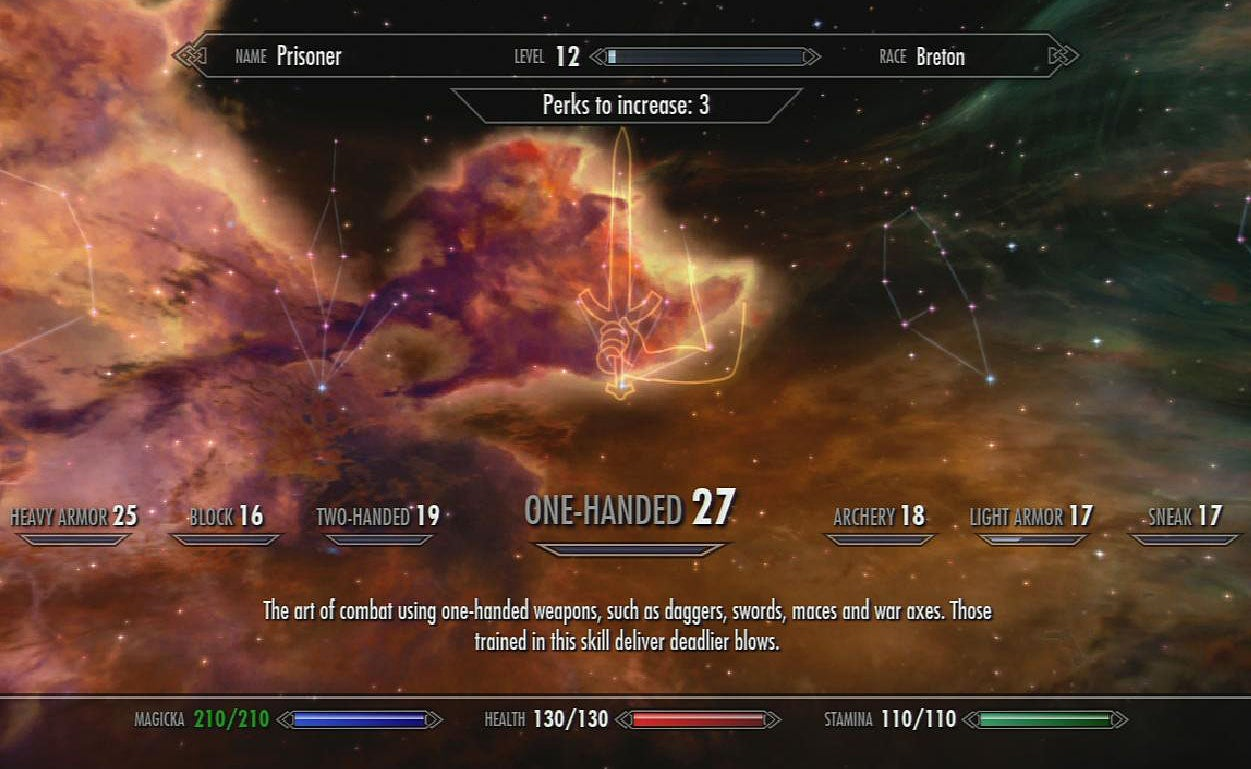
\includegraphics[width=1.0\textwidth]{images/tes.jpg}
\caption{Ekran rozwoju postaci z gry TESV:Skyrim.}
\end{figure}
